% 
%  chapter5.tex
%  ThesisISEL
%  
%  Created by Serge Lage on 2019/07/30.
%
% ================
% = Introduction =
% ================
\chapter{Joined Fishery Analysis}
\label{cha:server}
This chapter explains the approach used to reach the second goal of this work. 


Data mining is the process of discovering interesting and useful patterns and relationships in large volumes of data. The field combines tools from statistics and artificial intelligence (such as neural networks and machine learning) with database management to analyze large digital collections, known as data sets. Data mining is widely used in business (insurance, banking, retail), science research (astronomy, medicine), and government security (detection of criminals and terrorists) \cite{Okonkwo2011COMBATINGCA}. 

\section{CRISP-DM} % (fold)
\label{sub:crisp_dm}

In this work, it will be used the CRISP-DM (Cross Industry Standard Process for Data Mining) methodology \cite{CRISPDM}.
The CRISP-DM project proposed a comprehensive process model for carrying out data mining projects. The process model is independent of both the industry sector and the technology used \cite{CRISPDM}. 
The CRISP-DM reference model for data mining provides an overview of the life cycle of a data
mining project. It contains the phases of a project, their respective tasks, and their outputs.
The life cycle of a data mining project is broken down into six phases which are shown in Figure \ref{fig:crisp_dm}.
The sequence of the phases is not strict. The arrows indicate only the most important and frequent
dependencies between phases, but in a particular project, it depends on the outcome of each phase
which phase, or which particular task of a phase, has to be performed next.

\begin{figure}[H]
    \centering
    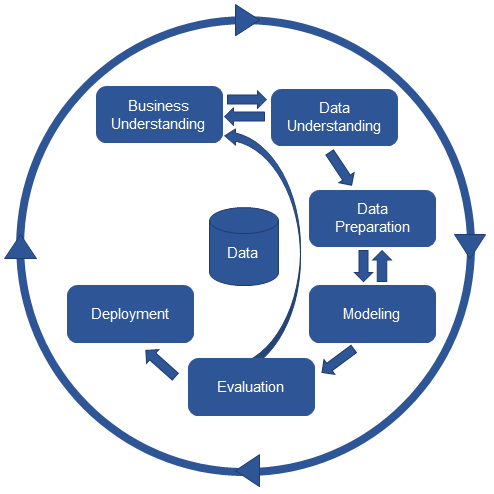
\includegraphics[width=0.8\linewidth]{Chapters/img/crisp_dm.png}
    \caption{Complete CRISP-DM Approach.}
    \label{fig:crisp_dm}
\end{figure}

In the following, we outline each phase briefly:
\begin{itemize}
\item Business Understanding\\
This initial phase focuses on understanding the project objectives and requirements from a
business perspective, and then converting this knowledge into a data mining problem
definition, and a preliminary project plan designed to achieve the objectives.
\item  Data Understanding\\
The data understanding phase starts with an initial data collection and proceeds with activities
to get familiar with the data, to identify data quality problems, to discover first
insights into the data, or to detect interesting subsets to form hypotheses for hidden
information.
There is a close link between Business Understanding and Data Understanding. The
formulation of the data mining problem and the project plan require at least some
understanding of the available data.
\item  Data Preparation\\
The data preparation phase covers all activities to construct the final dataset (data that will be
fed into the modeling tool(s)) from the initial raw data. Data preparation tasks are likely to be
performed multiple times, and not in any prescribed order. Tasks include a table, record, and attribute selection, data cleaning, construction of new attributes, and transformation of data for
modeling tools.
\item Modeling\\
In this phase, various modeling techniques are selected and applied, and their parameters are
calibrated to optimal values. Typically, there are several techniques for the same data mining
problem type. Some techniques require specific data formats.
There is a close link between Data Preparation and Modeling. Often, one realizes data
problems while modeling or one gets ideas for constructing new data.
\item Evaluation
At this stage in the project, you have built one or more models that appear to have high quality,
from a data analysis perspective. Before proceeding to the final deployment of the model, it is
important to more thoroughly evaluate the model, and review the steps executed to construct
the model, to be certain it properly achieves the business objectives. A key objective is to
determine if there is some important business issue that has not been sufficiently considered.
At the end of this phase, a decision on the use of the data mining results should be reached.
\item Deployment\\
The creation of the model is generally not the end of the project. Usually, the knowledge gained
will need to be organized and presented in a way that the customer can use it. Depending on
the requirements, the deployment phase can be as simple as generating a report or as complex
as implementing a repeatable data mining process. In many cases, it will be the user, not the
data analyst, who will carry out the deployment steps. In any case, it is important to
understand upfront what actions will need to be carried out to actually make use of
the created models.
\end{itemize}
% section crisp_dm (end)

\section{Implementation} % (fold)
\label{sub:implementation}

\subsection{Business Understanding} % (fold)
\label{sub:business_understanding}

In the fishing industry, vessels must have licenses to use fishing techniques.
The problem is that there is a probability that vessels are using fishing techniques or gear that is not licensed to do so.
The objective is to classify the VMS data by fishing type. 
In this way, we can try to confirm if each boat is carrying out the type of fishing for which it has the license paid.



% section business_understanding (end)


\subsection{Data Understanding} % (fold)
\label{sub:data_understanding}

The data we use for this objective are the same VMS Records as used in chapter 4 and VMS Vessels explained in chapter 3.2.
Let us focus on the use of speed, but not discriminating any of the remaining columns a prior without determining its potential in the contribution to a solution

% section data_understanding (end)



\subsection{Data Preparation} % (fold)
\label{sub:data_preparation}
To use data mining models, we need a dataset with all the data needed to feed the models. So, I created a dataset from VMS Vessels and VMS Records to end with Table \ref{table:vms_dataset}. 

\begin {table}[H]
\begin{center}
\begin{tabular}{c|c|c|c}
\textbf{Name }    & \textbf{Description} & \textbf{From} & \textbf{Why} \\
\hline
ID                & Key              & Native               & Identify the row           \\
VesselID          & Vessel Identifier   & VMS Records                & Identify the vessel  \\
UTC         & Date Time & VMS Records &Identify the time of the entry\\
LAT        & Latitude & VMS Records & Discriminated by fishing areas\\
LON        & Longitude & VMS Records & Discriminated by fishing areas\\
COG        & Direction & VMS Records & Course Over Ground\\
SOG        & Velocity & VMS Records & Discriminated by fishing velocity\\
LOA        & Length Overall & VMS Vessels & Discriminated by vessel type\\
GT        &  Gross Tonnage & VMS Vessels & Discriminated by vessel type\\
HP         &Vessel Power & VMS Vessels & Discriminated by vessel type\\
License        & Vessel's Linceses & VMS Vessels & Objective
           
\label{table:vms_dataset}
\end{tabular}
\caption {VMS Dataset}
\end{center}
\end {table}

%The License that occurs in the dataset are:
%\begin{itemize}
%\item    Armadilhas / De abrigo / Alcatruzes
%\item    Arrasto / De fundo de portas
%\item    Arrasto / De fundo de portas / Crustáceos
%\item    Arrasto / Pelágico / Com portas
%\item    Cerco / para bordo / Tipo americano
%\item    Emalhar de 1 pano / De deriva / Grandes Pelágicos
%\item    Emalhar de 1 pano / De fundo
%\item    Pesca à linha / Cana e linha de mão
%\item    Pesca à linha / Palangre de fundo / Espécies demersais
%\item    Pesca à linha / Palangre de Fundo + Cana e linha de mão
%\item    Pesca à linha / Palangre de superfície / Grandes Migradores
%\item    Tresmalho / De fundo
%\end{itemize}


The first thing to test is the correlation of the data to check if licenses are strongly correlated to some of the other variables. Figure \ref{fig:data_coor1} (the method used to find correlation was Pearson Correlation \cite{Benesty2009} that measures the degree of correlation and the direction of this correlation - whether positive or negative) between two metric scale variables). We can see that we can’t use the data as it is because de correlation between License and sog is very weak so we need to do some pre-processing.
\begin{figure}[h]
    \centering
    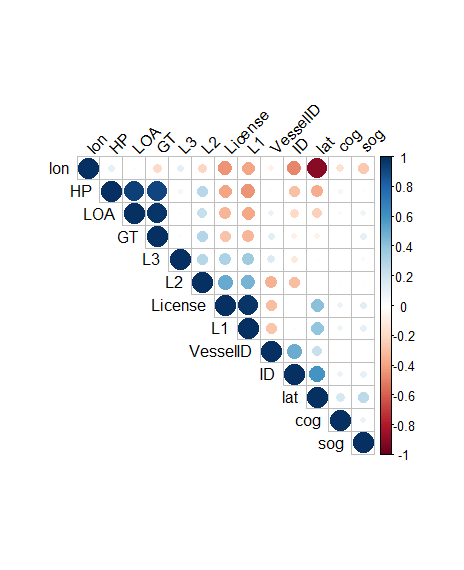
\includegraphics[width=0.7\linewidth]{Chapters/img/data_coor1.png}
    \caption{Data Correlation}
    \label{fig:data_coor1}
\end{figure}




The best way to achieve a greater correlation between fishing speeds and licenses was the transformation of data to storage fishing average, maximum and minimum per day per vessel. This way it presents the results shown in Figure \ref{fig:data_coor2}.

\begin{figure}[h]
    \centering
    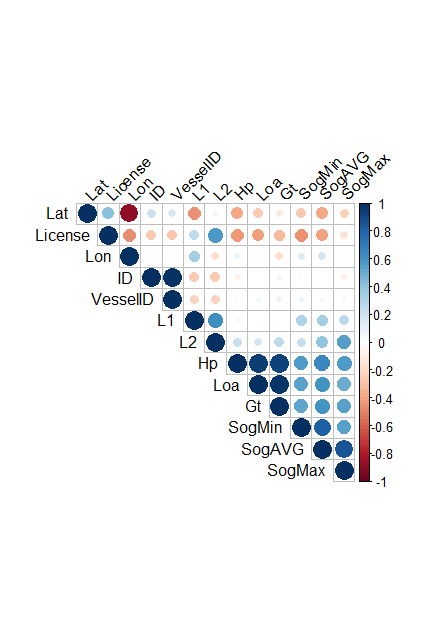
\includegraphics[width=0.7\linewidth]{Chapters/img/data_coor2.png}
    \caption{Data correlation after preprocessing}
    \label{fig:data_coor2}
\end{figure}
\newpage
The method used to transform the data consists of the following steps:
\begin{itemize}
\item    Create a dataset in which data are grouped per day, per vessel.
\item    Use DSALib to get the minimum and maximum speeds of fishing for poop vessels. With this data, filter the dataset to be only with data in which the speed of the vessel is between the minimum and maximum obtained.

\end{itemize}

With this data, we can also observe that the correlation between the license and the HP data (vessel power), Loa (Boat length) Gt (vessel weight) are quite significant. This is normal as different fishing activities require specific types of vessels. This does not mean that the type of vessel is only capable of entering a type of fishing activity.
For these reasons, I will not use these variables in the model so as not to create a problem with bias.
\\
Regarding location data, we used clustering techniques to discretize the data.
First, we need to know what the best number of clusters is. For that, we used the same technique used in chapter 4.3 with the output in Figure \ref{fig:elbow_method_server}. The data used was the dataset filtered so we have only the positions of fishing. The chosen number of clusters was 4.

\begin{figure}[H]
    \centering
    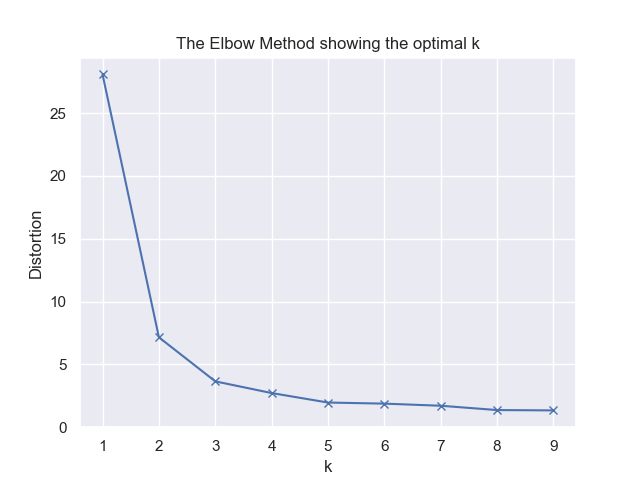
\includegraphics[width=0.8\linewidth]{Chapters/img/elbow_method_server.png}
    \caption{The elbow method showing the optinal k}
    \label{fig:elbow_method_server}
\end{figure}
Now we can create data mining models with location and velocity parameters.


% section data_preparation (end)
\newpage
\subsection{Modeling} % (fold)
\label{sub:modeling}
Several data mining algorithms were used to create the necessary models to classify the license type with the VMS data.
\begin{itemize}
\item \textbf{ KMeans:} This model was used in the previous step with the GPS data, so it was classified in well-defined clusters to improve the operation of the data mining algorithms. The operation of this algorithm is described in chapter 4.3.

\item \textbf{ Decision Trees: }
While in data mining a decision tree is a predictive model that can be used to represent both classifiers and regression models, in operations research decision trees refer to a hierarchical model of decisions and their consequences. The decision-maker employs decision trees to identify the strategy which will most likely reach its goal. When a decision tree is used for classification tasks, it is most commonly referred to as a classification tree. When it is used for regression tasks, it is called a regression tree \cite{Rokach2014}.
Algorithms for constructing decision trees usually work top-down, by choosing a variable at each step that best splits the set of items \cite{ApplicationsReviews}.\\
In this work it will be used to measure the quality of a split "gini" for the Gini impurity (CART)\cite{DTAnalysis} and "entropy" for the information gain (C4.5)\cite{DTAnalysis}.

\item \textbf{ Random Forests: }
Random forests are a combination of tree predictors such that each tree depends on the values of a random vector sampled independently and with the same distribution for all trees in the forest\cite{Breiman2001}. The generalization error for forests converges a.s. to a limit as the number of trees in the forest becomes large. The generalization error of a forest of tree classifiers depends on the strength of the individual trees in the forest and the correlation between them.
A random forest is a classifier consisting of a collection of tree-structured
classifiers \(\{h(\textbf{x}, \theta \textsubscript{k} ), k = 1,...\}\) where the  \( \{ \theta \textsubscript{k} \}\) are independent identically distributed
random vectors and each tree casts a unit vote for the most popular class at input \textbf{x}\cite{Breiman2001}.


\item \textbf{Neural Network: }
Neural networks are a bio-inspired mechanism of data processing, that enables computers to learn technically similar to a brain and even generalize once solutions to enough problem instances are tough \cite{Kriesel2007NeuralNetworks}. A technical neural network consists of simple processing units, the neurons, and directed, weighted connections between those neurons. A neural network is a sorted triple \((N, V, \varpi )\) with two sets N, V and a  function \(\varpi\), where N is the set of neurons and V a set \(\{ (i, j) i, j \in \mathbb{N} \}\)  whose elements are called connections between neuron i and neuron j. The function \( \varpi : V \rightarrow \mathbb{R}\) defines the weights, where \(\varpi((i, j))\), the weight of the connection between neuron \(i$ and neuron \(j$, is shortened to \(\varpi \textsubscript{ i,j}\) . Depending on the point of view it is either undefined or 0 for connections that do not exist in the network \cite{Kriesel2007NeuralNetworks}.  \\
In this work we will train models with different hidden layer sizes. The solver for weight optimization used is BFGS\cite{Dai2013} and Adam\cite{adamNN} for large sizes of hidden layers.

\item \textbf{Support Vector Machine: }
The folklore view of SVM is that they find a \"optimal\" hyperplane as the solution to the learning problem. The simplest formulation of SVM is the linear one, where the hyperplane lies in the space of the input data \(x\). In this case, the hypothesis space is a subset of all hyperplanes of the form:
\(f(x) = w \cdotp x +b\).
In their most general formulation, SVM finds a hyperplane in a space different from that of the input data x. It is a hyperplane in a feature space induced by a kernel K (the kernel defines a dot product in that space)\cite{SVMEvgeniou}.\\
In this work we will create models using the following kernel algorithms: Linear\cite{SVMTraining}, Polynomial\cite{SVMTraining} and RBF\cite{SVMTraining}.  
\end{itemize}






% section modeling (end)

\subsection{Evaluation} % (fold)
\label{sub:evaluation}
Cross \textendash validation \cite{CrossValidatory} provides a simple and effective method for both model selection and performance evaluation, widely employed by the machine learning community. Under k \textendash fold cross \textendash validation the data are randomly partitioned to form k disjoint subsets of approximately equal size. In the ith fold of the cross-validation procedure, the ith subset is used to estimate the generalization performance of a model trained on the remaining k \textendash 1 subset. The average of the generalization performance observed overall k folds provides an estimate (with a slightly pessimistic bias) of the generalization performance of a model trained on the entire sample.
The k used to test these models is 10.
The method used in this work to evaluate the models are:\\
Precision = \(\sum_{n=0}^{k-1}\frac{tp}{tp+fp} \)  = precision of the model.\\
Accuracy = \( \sqrt{precision} ^ 2\) = accuracy of the precision result.\\


A confusion matrix \cite{CMPatil} illustrates the accuracy of the solution to a classification problem. Given n classes, a confusion matrix is a m x n matrix, where C\textsubscript{i,j} indicates the number of tuples from D that were assigned to class C\textsubscript{i,j} but where the correct class is C\textsubscript{i}.
Obviously, the best solution will have only zero values outside the diagonal.
A confusion matrix contains information about actual and predicted classifications done by a classification system. The performance of such systems is commonly evaluated using the data in the matrix. The following table shows the confusion matrix for a two-class classifier. 

For the propose of this work, the classes are: 

0    Armadilhas / De abrigo / Alcatruzes \\
1    Arrasto / De fundo de portas \\
2    Arrasto / De fundo de portas / Crustáceos\\
3    Arrasto / Pelágico / Com portas\\
4    Cerco / para bordo / Tipo americano\\
5    Emalhar de 1 pano / De deriva / Grandes Pelágicos\\
6    Emalhar de 1 pano / De fundo\\
7    Pesca à linha / Cana e linha de mão\\
8    Pesca à linha / Palangre de fundo / Espécies demersais\\
9    Pesca à linha / Palangre de Fundo + Cana e linha de mão\\
10    Pesca à linha / Palangre de superfície / Grandes Migradores



The model's test results are:
\newpage
\begin{itemize}
\item \textbf{ Decision Trees: }

We can observe in Table \ref{table:cross_val_dt} the usage of velocity parameters (SogMin, SogAVG, and SogMax) and location (clustering result of K-Means) have the best result. The algorithm with the best result is Entropy(C4.5) with a precision of 0.7776 and an accuracy of 0.1459. In Figure \ref{table:cross_val_dt} the confusion matrix shows that only the classes 0 and 7 have a low prediction rate. The max depth of the trees was tested as 200, 300 and 400 with 300 giving the best results.


\begin {table}[H]
\begin{center}
\begin{tabular}{c|c|c|c|c}
\multicolumn{1}{c|}{\textbf{Algorithm } }   &\multicolumn{2}{c|}{\textbf{ Velocity and locations}}& \multicolumn{2}{c}{\textbf{ Velocity}}\\
&Precision & Accuracy & Precision & Accuracy \\
\hline
Gini   &0.774&0.1481&0.7236&0.1349\\
Entropy&0.7776&0.1459&0.73&0.1319
\label{table:cross_val_dt}
\end{tabular}
\caption {Cross-Validation results for Decision Trees models}
\end{center}
\end {table}

\begin{figure}[h]
    \centering
    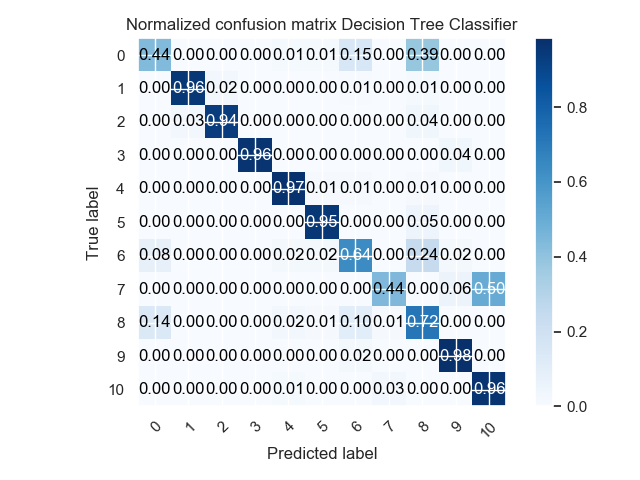
\includegraphics[width=0.8\linewidth]{Chapters/img/CM_DT.png}
    \caption{Confusion Matrix for Decision Tree using Entropy(C4.5)}
    \label{fig:cm_dt}
\end{figure}


\newpage
\item \textbf{ Random Forest: }

In this models it was trained with the algorithms of Gini and Entropy(C4.5) with the same result of Decision trees, the Entropy was a better precision. So the results mentioned in this document for Random Forest models are using Entropy(C4.5) as the algorithm to measure the quality of a split. The max depth of the trees was tested as 200, 300 and 400 with 300 giving the best results. In table \ref{table:cross_val_rf} we can see that the best result was given by the model with 200 estimators.In Figure \ref{table:cross_val_rf} the confusion matrix shows that only the classes 0 and 7 have a low prediction rate. 


\begin {table}[H]
\begin{center}
\begin{tabular}{c|c|c|c|c}
\multicolumn{1}{c|}{\textbf{No. of estimators } }   &\multicolumn{2}{c|}{\textbf{ Velocity and locations}}& \multicolumn{2}{c}{\textbf{ Velocity}}\\
&Precision & Accuracy & Precision & Accuracy \\
\hline
50  &0.8097&0.1355 &0.7649 &0.1315\\
100 &0.8082&0.1332 &0.7684 &0.133\\
200 &0.8101&0.1436 &0.767  &0.1337 \\
300 &0.8075&0.1458 &0.771 &0.1339 
\label{table:cross_val_rf}
\end{tabular}
\caption {Cross-Validation results for Random Forest models}
\end{center}
\end {table}


\begin{figure}[h]
    \centering
    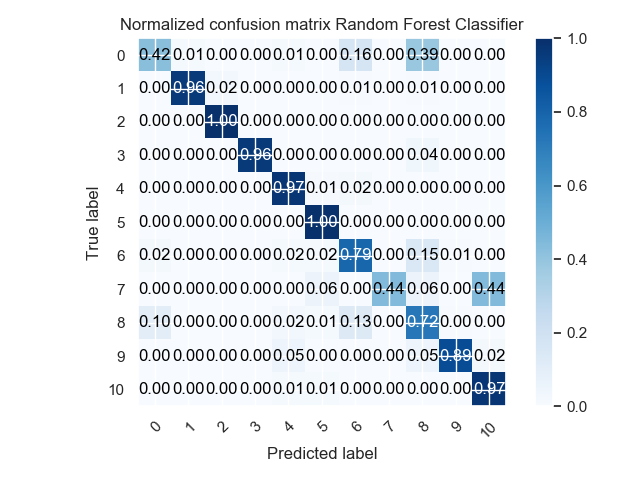
\includegraphics[width=0.8\linewidth]{Chapters/img/CM_RF.png}
    \caption{Confusion Matrix for Random Forest using 200 estimators}
    \label{fig:cm_rf}
\end{figure}


\newpage
\item \textbf{Neural Network: }\\
For this models it was trained various configurations of hidden layers. It was used from 1 to 8 hidden layers with 11, 250, 500 and 750 neurons. Some of the results are in Table \ref{table:cross_val_nn}. The best result as we can observe in Table \ref{table:cross_val_nn} as 5 layers with 500 neurons with the confusion matrix represented in Figure \ref{fig:cm_nn}.
For some models it was used the Adam solver and BFGS, but with BFGS having better results. So all results demonstrated are using BFGS solver.
As in Decision Trees models, the usage of locations have a good impact in the results of the Neural Network models.


\begin {table}[H]
\begin{center}
\begin{tabular}{c|c|c|c|c}
\multicolumn{1}{c|}{\textbf{Hidden Layers } }   &\multicolumn{2}{c|}{\textbf{ Velocity and locations}}& \multicolumn{2}{c}{\textbf{ Velocity}}\\
&Precision & Accuracy & Precision & Accuracy \\
\hline
None &0.6293&0.147   &0.5984 &0.1359\\
11   & 0.6569&0.1531   &0.644 &0.1258\\
4 500 &0.7054&0.1479  & 0.0657 & 0.1674\\
5 500 & 0.7654&0.1535 &0.7309 & 0.1286\\
6 500 &0.7642 &0.1421 &0.7299 &0.1291 
\label{table:cross_val_nn}
\end{tabular}
\caption {Cross-Validation results for Neural Network models}
\end{center}
\end {table}


\begin{figure}[h]
    \centering
    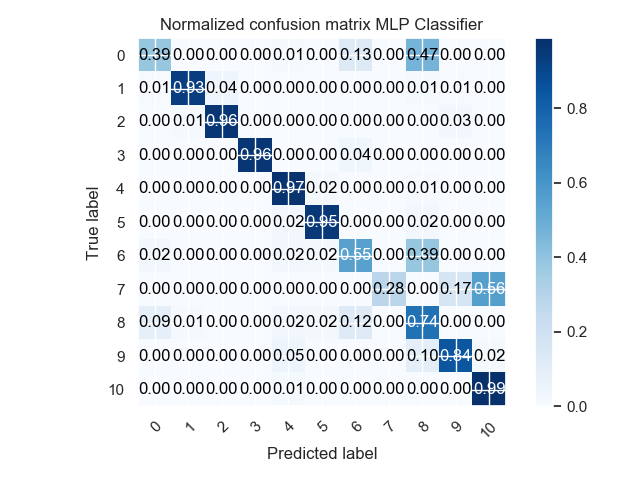
\includegraphics[width=0.8\linewidth]{Chapters/img/CM_NN.png}
    \caption{Confusion Matrix for Neural Network using 5x500 hidden layers}
    \label{fig:cm_nn}
\end{figure}


\newpage
\item \textbf{Support Vector Machine: }\\
For the built of support vector machine models it was used the kernel coefficient of Polynomial, RBF and linear. With the best result as we can observe in Table \ref{table:cross_val_svm} is the Polynomial, with its confusion matrix represented in Figure \ref{fig:cm_cvm}.  



\begin {table}[H]
\begin{center}
\begin{tabular}{c|c|c|c|c}
\multicolumn{1}{c|}{\textbf{Kernel coefficient } }   &\multicolumn{2}{c|}{\textbf{ Velocity and locations}}& \multicolumn{2}{c}{\textbf{ Velocity}}\\
&Precision & Accuracy & Precision & Accuracy \\
\hline
Polynomial    &0.702 &0.0848    & 0.6573&0.108\\
RBF     &0.697&0.1092  & 0.6611&0.12\\
Linear  &0.6018&0.0746  & 0.5192&0.0263
\label{table:cross_val_svm}
\end{tabular}
\caption {Cross-Validation results for Support Vector Machine models}
\end{center}
\end {table}

\end{itemize}

\begin{figure}[h]
    \centering
    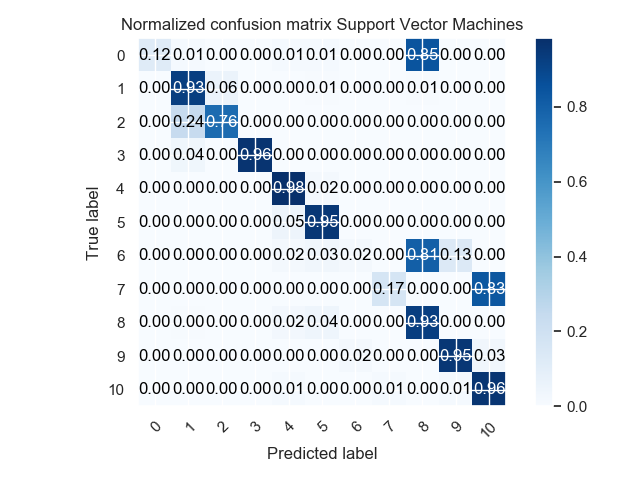
\includegraphics[width=0.8\linewidth]{Chapters/img/CM_SVM.png}
    \caption{Confusion Matrix for Support Vector Machine using Polynomial kernel coefficient}
    \label{fig:cm_cvm}
\end{figure}


\newpage
The model with best result was Random Forest with 200 estimators with a precision of 81.01\% (accuracy of the evaluation is 0.1436).
With this we can determine that it is possible to create a good model to classify the VMS data as the fishing license. \\
As seen in Figure \ref{fig:cm_rf}, the classes 0 and 7 have a low true positive rate. The usage of more data and data that are certified that the VMS data of a vessel is only for the propose of the fishing license can improve the precision of the model.


%Determine Next Steps
%List of Possible Actions
%Decision

% section evaluation (end)


\subsection{Deployment} % (fold)
\label{sub:deployment}
Joined Fishery Analysis

%Plan Deployment Deployment Plan

%Plan Monitoring andMaintenance
%Monitoring and Maintenance Plan

%Produce Final Report
%Final Report
%Final Presentation

%Review Project
%Experience
%Documentation
% section deployment (end)

% chapter server (end)



